% vim: set tw=78 sts=2 sw=2 ts=8 aw et ai:
\documentclass[12pt]{article}

\usepackage[paper=a4paper, top=2cm, bottom=3cm, left=2.5cm, right=2.5cm]{geometry}

\usepackage{ucs}
\usepackage[utf8x]{inputenc}
\usepackage[english]{babel}
%\usepackage{hyperref}	  % use \url{http://$URL} or \href{http://$URL}{Name}
\usepackage{underscore}	  % underscores need not be escaped
\usepackage{subfigure}
\usepackage{verbatim}
\usepackage{float}
\usepackage{booktabs}     % professional tables
\usepackage{parskip}

% Support for including graphics
\usepackage{graphicx}
\DeclareGraphicsExtensions{.pdf,.png,.jpg}

\title{FPGA acceleration of Machine Learning (ANN training and inference)}

\author{Alexandru Rares Apostol\\
Faculty of Electronics, Telecommunications and Information Technology\\
University POLITEHNICA of Bucharest\\
Splaiul Independenței 313, Bucharest, Romania, 060042 \\
\emph{alexandru.apostol@upb.ro}}

\date{\today}

\begin{document}

\maketitle

\begin{abstract}
% vim: set tw=78 sts=2 sw=2 ts=8 aw et ai:

Due to the rapid evolution of digital technologies, the area of deep learning artificial neural networks has demonstrated its ability and  effectiveness in solving complex learning problems of various engineering applications. However, they require intensive CPU operations and memory bandwidth that ultimately lead the CPUs to very low performance levels with respect to execution speed. Consequently, hardware accelerators that make use of application specific integrated circuits (ASICs), field programmable gate arrays (FPGAs) and graphic processing units (GPUs) have been selected to improve the overall performance of an ANN application. More precisely, FPGAs have been recently adopted for accelerating the implementation of deep learning networks due to their ability to maximize parallelism as well as due to their energy efficiency. 
In this paper, a review of the recent existing techniques for accelerating ANNs on FPGAs is performed. It presents the key features that are being used by the various techniques that improve the acceleration performance. The techniques presented in this paper represent the recent trends in FPGA-based accelerators of artificial neural networks. \\
\textbf{Keywords:} NN, ANN, FPGA, Machine Learning

\end{abstract}

\section{Introduction}
\label{sec:introduction}
% vim: set tw=78 sts=2 sw=2 ts=8 aw et ai:

Artificial Neural Networks (ANNs) are computing systems in machine learning inspired by the biological neural networks that constitute the animal brain. As such, they have been variously used in applications that require memory mapping, classification, clustering, pattern recognition etc. ANNs are one type of model for machine learning (ML) and has become relatively competitive to conventional regression and statistical models regarding usefulness \cite{ANNreview}. In most applications, artificial neural networks have been implemented in software. This presents its own benefits, due to the fact that the designer/developer does not need to know the hardware component of the application and can concentrate on the software component. However, a major disadvantage that occurs in software based ANNs is that their performances are lower with respect to execution time when compared with hardware-based ANNs.

Hardware-based ANNs have been developed and implemented as both digital and analogue circuits. While the analogue ANNs explore the nonlinear characteristics of the CMOS (complementary metal-oxide semiconductor) devices, the digital component explores the implementation of large ANNs on a single FPGA device in order to overcome the calculation complexity of software implementations. As the analogue implementation tends to suffer from thermal drift, inexact computation results and lack of reprogrammability, the digital implementation is commonly used \cite{efficientDigitalImpl}.

\section{Artificial Neural Network}
\label{sec:artificialNeuron}
% vim: set tw=78 sts=2 sw=2 ts=8 aw et ai:

\subsection{Artificial Neuron}
Artificial neural networks are inspired by the biological neural systems. The transmission of signals in biological neurons through synapses is a complex chemical process in which specific transmitter substances are released from the sending side of the synapse. The desire is to change the logical level of the receiving cell. 

\begin{figure}[H]
    \centering
    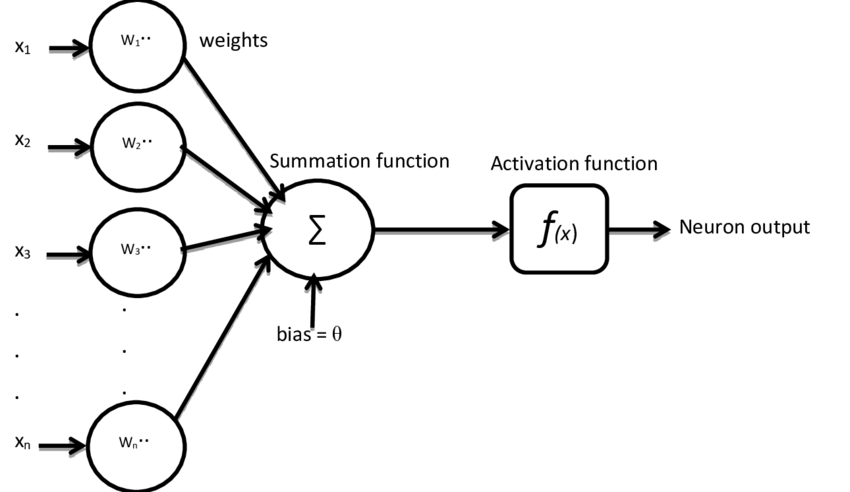
\includegraphics[width=0.7\linewidth]{img/artificialNeuron.png}
    \caption{Artificial neuron structural diagram\cite{impactANN}}
    \label{fig:artificialNeuron}
\end{figure}

The artificial neuron presented in the figure above has N inputs, each input being assigned a weight, denoted as $w_1, w_2...w_N$. The activation $y$ determines if the neuron is to be fired or not. It can be represented with the following formula:

\begin{equation}
    y=\sum_{i=1}^nw_ix_i
\end{equation}

\subsection{Neural network structure}
A neural network system consists of a varying number of artificial neurons and a very large number of interconnections. In a neural network, single neurons are arranged in layers. The manner in which they are arranged in a layer and how the connections are being executed with the next layer indicates the type of network in use. The three major important neural network types are:

\begin{itemize}
    \item Feed-forward of fully connected (FC) neural networks.
    \item Convolutional neural netrowks (CNNs)
    \item Recurrent neural networks (RNNs).
\end{itemize}

\begin{figure}[H]
    \centering
    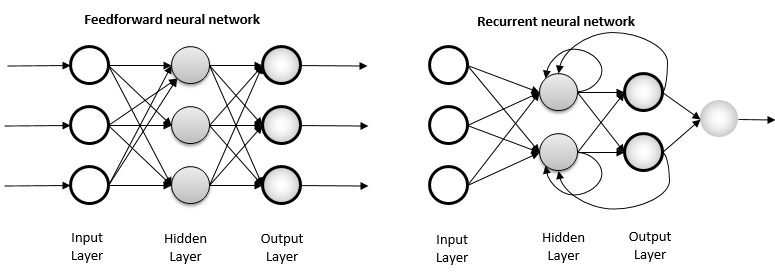
\includegraphics[width=0.8\linewidth]{img/feedForwardRecurrent.png}
    \caption{Examples of neural network architectures\cite{layersFigure}}
    \label{fig:layersFigure}
\end{figure}

In layered neural networks, the neurons are organized in the form of layers. The neurons in one layer get input from the previous layer and feed their output to the next layer. The layers which are processing the data are called hidden layers. The output layer is the last layer of a neural network and provides the results of a neural network. Usually, the output of a neural network is represented in the form of a probability of specific possible results. Each layer contained in a feed-forward layer is described by Equation (1), whilst the weight matrix $w_i$ contains an entry for each neuron connected between two layers. Networks with one or more hidden layers are called multi-layer networks.

\subsection{Inference and Training}

In most applications, ANNs are deployed in two phases. The first deployed stage is the training stage in which a known set of annotated data samples are used in order to create a model. When training, ANN models can be fine-tuned. When fine-tuning a model, weights of a previously-trained network are used to initialize the parameters of a new training. These weights may be adjusted for new constraints, such as a different dataset, reduced precision etc.

The second phase, known as inference, makes use of the learnt model to classify new data samples (i.e. inputs that were not previously seen by the model). In a typical setup, ANNs are trained and fine-tuned only once. The inference is implemented every time a new data sample needs to be classified. 

\section{Field-Programmable Gate Arrays}
\label{sec:fpgaVerilog}
Field-Programmable Gate Arrays (FPGAs) are readily available, multi-sourced components which have a proven place in development, small-scale production, and even large-scale production runs. 
Its impressive properties, such as high computational speed and intrinsic parallelism, are crucial in most of the experiments and applications performed nowadays.
Many application programs demand more processing power than can be supplied by conventional processing resources. Many of these programs have a kernel which is responsible for a significant fraction of the total execution time of the program. 

\subsection{Architecture}
FPGAs consist of an array of programmable logic blocks of potentially different types, including general logic, memory and multiplier blocks, surrounded by a programmable routing fabric that allows blocks to be programmably interconnected. The array is surrounded by programmable input/output blocks that connect the chip to external devices\cite{fpgaStructureBook}.

\begin{figure}[H]
    \centering
    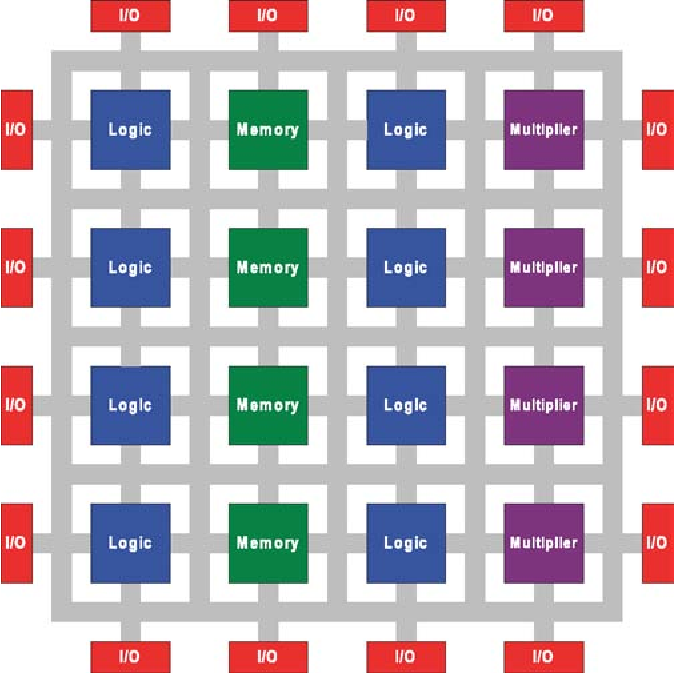
\includegraphics[width=0.5\linewidth]{img/fpgaStructure.png}
    \caption{Basic FPGA structure\cite{fpgaStructureBook}}
    \label{fig:fpgaStructure}
\end{figure}

\subsection{FPGA as hardware accelerators}
FPGAs usually operate at lower clock frequencies than ASICs (Application Specific Integrated Circuits) and ASSPs (Application-Specific Standard Products), but they are very customizable and present multiple advantages:
\begin{itemize}
    \item Implementing wider parallelism in hardware
    \item Easily changing the size of data
    \item Provides an easy and inexpensive way to modify the neural network.
    \item Experimentation with alternative circuits makes them very attractive for both prototyping and new products.
\end{itemize}
The main disadvantage when it comes to using FPGAs is the price. FPGAs are more expensive than the majority of widely used microprocessors. For some applications, microprocessors also perform better. Thus, FPGAs are relevant for only a set of high-performance computations and algorithms.

Hardware accelerators are, as a rule, non-autonomous circuit that has to interact with some other circuits, and yields better performances as more items are handled in parallel.

\section{Accelerating ANNs on FPGAs}
\label{sec:accelAnnFpga}
In order to accelerate the execution of ANN, FPGAs have been considered and researched. In recent years, numerous FPGA designs for ANN training and inference have been proposed with the key objective of designing a system that provides high energy efficiency while mainaining low latencies. This section numerous strategies are being summarized in order to identify the best approach when selecting and designing an FPGA that provides efficient ANN acceleration.

\subsection{Algorithmic Optimization}

Algorithmic optimization applies computational transformation or vectorization of data in order to reduce the number of performed arithmetic operations and memory accesses. Mainly CPUs and GPUs use these techniques. However, various FPGAs based neural network implementations are using algorithmic optimization\cite{CnnFpgaSurvey}.

\subsubsection{General Matrix Multiplication}
The general matrix multiplication algorithm (GEMM) minimizes the required memory accesses for vector-matrix multiplications by using same-weight multiplications into a vector. The main advantage of this method is that a single weight is fetched only once. The figure below visualizes that the reuse of a weight matrix increases by a factor of N for N batches.

\begin{figure}[H]
    \centering
    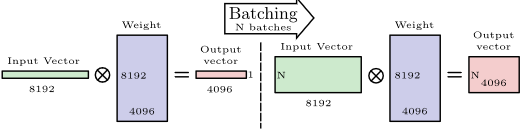
\includegraphics[width=0.7\linewidth]{img/batching.png}
    \caption{Batching that converts vector matrix multiplication into matrix-matrix multiplication\cite{learningOnHardware}}
    \label{fig:batching}
\end{figure}

For feed-forward layers, batching increases the utilization of single instruction multiple data (SIMD) processors\cite{CnnAdvances}. However, if real-time applications use batching, it has to be ensured that the latency requirements are not violated, since batching may increase the latency\cite{CnnAdvances}.

\subsubsection{Fast Fourier Transformation}
\begin{figure}[H]
    \centering
    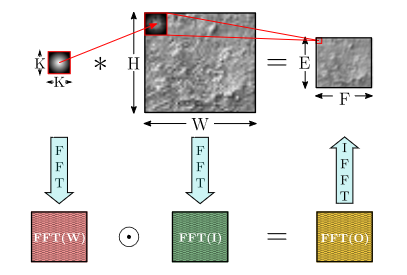
\includegraphics[width=0.7\linewidth]{img/fft.png}
    \caption{Fast Fourier Transformation\cite{efficienfProcessingDnn}}
    \label{fig:fft}
\end{figure}

The Fast Fourier Transform is a well known algorithm that reduces the arithmetic complexity from 
$O(N_K^2N_O^2)$ to $O(N_O^2log_2(N_O))$, with $N_K \times N_K$ is the filter size and $N_O \times N_O$ is the output size\cite{efficienfProcessingDnn}.

However, there are several drawbacks to using FFT:
\begin{enumerate}
    \item The benefits of FFTs decrease with filter size.
    \item The size of the FFT is dictated by the output feature map size which is often much larger than the filter.
    \item The coefficients in the frequency domain are complex
\end{enumerate}
As a result, while FFT reduces computation, it requires larger storage capacity and bandwidth. Also, since modern neural networks mainly use small filter sizes FFT has lost importance in modern hardware accelerators.

\subsection{Accelerating Nested Loops}
When designing a neural network hardware accelerator, the main idea is to parallelize operations. From an algorithmic point of view, matrix computations can be seen as nested loops. There are a number of approaches in order to accelerate the computation of these loops:
\begin{itemize}
    \item Loop recording
    \item Loop unrolling
    \item Loop pipelining
    \item Loop tiling
\end{itemize}
When using matrixes, efficient memory allocation must also be taken into consideration; loop tiling is used for partitioning.\cite{CnnFpgaSurvey2}

\subsubsection{Loop Recording}
The main goal is to avoid redundant memory accesses and maximize cache usage efficiency while decreasing the computation time\cite{CnnFpgaSurvey2, CnnAdvances}. This can result in significant differences in performance\cite{CnnAdvances}.

\subsubsection{Loop unrolling}
Independent loops can be executed simultaneously by using parallel hardware. The main goal is to decrease the computation time by increasing the hardware utilization\cite{CnnFpgaSurvey2, CnnAdvances}.

\subsubsection{Loop pipelining}
The goal is to divide the nested loops into sequential steps, which can be performed in parallel\cite{CnnAdvances}. The implementation of pipelining is dependent on the architecture of the hardware accelerator.

\subsubsection{Loop tiling}
Loop tiling partitions the cache into tiles, which load as a whole chunk from memory, to avoid the data in the cache to supersede before the usage\cite{CnnAdvances}. In terms of ASICs and FPGAs, loop tiling refers to the efficient usage of the available on-chip memory.

\subsection{ANN compression methods}
To narrow the gap between accuracy requirement and hardware performance whilst increasing computational efficiency, two approaches are usually followed and implemented:
\begin{itemize}
    \item Quantization
    \item Pruning
    \item Knowledge Distillation
\end{itemize}

\subsubsection{Weight and Data Quantization}
Several methods have been proposed to quantize the NN weights after training, using 16-bit\cite{deepLearningLimitedNumericalPrecision} and 8-bit\cite{8BitApprox} fixed point representation, which presented slight but not dramatic improvements with respect to classification accuracy. However, logarithmic quantization\cite{NetworkQuantization} has provided a significant more efficient inference, when each quantization point is a power of two as fixed-point multiplication can be replaced with bit shift operations that correspond to the power of two.
In addition to weight quantization, data quantization is quintessential with respect to efficiency improvement. Data quantization reduces the cost of memory access for intermediate output layers\cite{NetworkQuantization} in a multiple layer ANN and also the computation cost of inference. However, low precision quantization of activation (i.e. 1-4 bits) leads to a significant degradation in classification accuracy when being compared to weight quantization\cite{weightsActivationsConstrained}. Due to these considerations, the trend is to use 8-bit linear quantization.

\subsubsection{Weight Pruning}
The majority of weights in an ANN (up to 90\% for large models) may be pruned (set to zero) without providing a significant impact on the accuracy of the classification. A pruned ANN may provide sparsely distributed weights with an irregular sparsity structure, which is generally difficult to implement in an efficient manner using conventional hardware such as the GPU\cite{deepCompression}. The main advantage of pruning consists of reduced disk storage and computational effort. However, when pruning, retraining of the neural network is required in order to avoid accuracy loss\cite{learningOnHardware}.
Pruning can be executed through various methods:
\begin{itemize}
    \item Fine-grained pruning in which any weight that finds to be unimportant will be pruned.
    \item Vector and kernel-level pruning where pruning is constrained to vectors of the neural network
    \item Group-level pruning in which a filter that can be inputted in the neural network will act as the pruning method.
    \item Filter-level pruning in which the pruning method focuses on reducing the dimension of a layer.
\end{itemize}

\subsubsection{Knowledge Distillation}
The main idea behind the knowledge distillation concept is that a single model will not be able to provide higher accuracy models when compared to the averaging predictions of different models. Since using multiple neural networks is not feasible since it will provide additional computational effort, knowledge distillation combines the knowledge of different networks into a newer, simpler model. Based on the output of the knowledge-providing neural networks, the new neural network's biases and weights are adjusted using stochastic gradient descent\cite{efficientProcessingNNSurvey}. As such, using knowledge distillation can provide the same or even more accurate prediction whilst keeping into account the computation efficiency factor.

\subsection{FPGA Hardware Architectures}
Most FPGA accelerators use one of the following 2 hardware structures: Single computation engines and streaming architectures\cite{mappingCnnFpga}.

\subsubsection{Single computation engines}
The single computation engines favours flexibility over customization and is usually implemented in a systolic array\cite{mappingCnnFpga} that executes ANN layers sequentially. The control of the hardware and the scheduling of operations if performed by software means. In a systolic array, each processing element can exchange data with the adjacent processing element, which enables the systolic array to have a high data rate. However, inputs, outputs and weights are being transferred to and from the external memory, which ultimately leads to a bottleneck.

\begin{figure}[H]
    \centering
    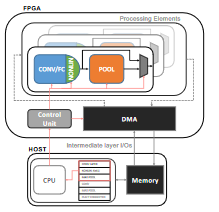
\includegraphics[width=0.4\linewidth]{img/singleComputationEngine.png}
    \caption{Single Computation Engine example\cite{mappingCnnFpga}}
    \label{fig:singleComputationEngine}
\end{figure}

The benefit of using systolic arrays is that they are easily adaptable for different ANN structures. However, this flexibility comes with the price of reduced efficiency, which may lead to different performance issues during an ANN application.

\subsubsection{Streaming architectures}
As opposed to the single computation engines, streaming architectures implement an independent and specialized processing elements for each layer. The data is pipelined through the hardware accelerator. Even so, the processing elements must be designed so that the calculations of each individual layer takes the same amount of processing time to avoid idling. The weights are stationary required for a specific layer, which reduces global data transfer\cite{learningOnHardware}. This enables the streaming architecture to implement a highly efficient accelerator. However, when being compared to the single computation engine architecture, they prove to be less flexible since they are mainly optimized for a single neural network structure\cite{learningOnHardware}.

\begin{figure}[H]
    \centering
    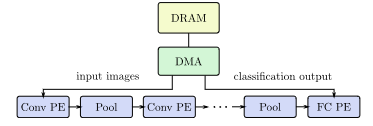
\includegraphics[width=0.7\linewidth]{img/streamingArhitecture.png}
    \caption{Streaming architecture example\cite{learningOnHardware}}
    \label{fig:streamingArchitecture}
\end{figure}

\subsection{Hardware accelerator implementations}

\subsubsection{32-bit floating-point single computation engine \cite{exampleFPGA2}}
In 2015 Zhang et al. introduced a 32-bit floating-point single computation engine on a high-end Xilinx FPGA using HLS. The accelerator uses 64 two-level unrolled processing elements operating with 100MHz. Each processing element has 7 inputs for activations and weights and 1 bias input. Additionally, buffers are applied to input and output. The size of the buffers on-chip is fixed using loop tiling. A MicroBlaze CPU controls the data flow of the hardware accelerator. The system has a power consumption of 18.61W. Due to the high precision processing elements, no accuracy loss occurs. However, the high precision results in a low throughput. For this reason, this design has compared to others a poor implementations efficiency.

\subsubsection{10-bit SIMD engine \cite{exampleFPGA1}}
In 2019 Sudarshan Srinivasan et al. implemented an FPGA-based accelerator with 8 bit activation and 2 bit weights. The FPGA architecture provided a highly configurable SIMD engine and the accelerator was written in RTL. The optimization methods selected by the authors were only the FPGA pipelining and quantization of data. It implemented the ResNet50 convolutional neural network. The paper presented a top-1 accuracy of 71.1\%. It efficiently implemented a ResNet50 network with 8-bit activations and ternary weights on an FPGA. The design is capable of performing 16K MAC operations per cycle.

\subsubsection{16-bit float-point single computation engine \cite{exampleFPGA3}}
Aydonat et al. use 16-bit floating-point operations for accumulation and 16 bit fixed point operation
for multiplication to reduce the overhead from using FP32 digital signal processings. The hardware accelerator structure uses serial processing elements, optimized for computing Winograd transformed feature maps. The Winograd approach that achieves over 60\% digital signal processing efficiency and uses the Winograd transform to significantly reduce the digital signal processings required to perform the convolution layers. 

\section{Conclusion}
\label{sec:conclusion}
% vim: set tw=78 sts=2 sw=2 ts=8 aw et ai:

In recent years, the accuracy yielded by neural networks is rapidly increasing. For this reason, neural networks are widely used for various applications. However, the increasing accuracy bases on an exponential expansion of the number and size of the variables used in the network, which ultimately leads to an exponential increase of the computational load. Such computational loads may be hard to handle by classical software neural networks. As a consequence, optimized neural networks hardware accelerators have been taken in consideration. Optimization can be achieved through various methods such as algorithmic operation, quantization, pruning etc. However, the target hardware accelerators architecture also plays a role in a network design. Some hardware elements may or may not support the implementation of the optimization solutions. Also, some optimization techniques increase performance whilst reducing accuracy.

FPGAs offer a programmable logic circuit that enables a highly optimized design with a relatively low design effort and initial costs. FPGA-based hardware accelerators widely use the algorithmic optimization methods described in this paper. However, depending on the structure of the hardware accelerator, the methods may yield different performances. For example, while the GEMM algorithm is well suited for FPGAs that support batching, it is not suited for streaming architectures since multiple batches would require an enormous tile size of the buffers. When using the FFT algorithm, it is more suitable for large filter sizes.

In conclusion, implementing neural networks on FPGAs is considered a feasible solution as it provides better performances, flexible architecture options and data flow optimization options while being easily reprogrammable and having a higher power efficiency.

\bibliographystyle{abbrv}
\bibliography{ref}

\end{document}
